\documentclass[mgr, shortabstract]{iithesis}

\usepackage[utf8]{inputenc}
\usepackage{amsmath}
\usepackage{minted}
\usepackage{listings}
\usepackage{graphicx}
\usepackage{lmodern}

%%%%% DANE DO STRONY TYTUŁOWEJ
\polishtitle    {Polski tytuł}
\englishtitle   {English title}
%\polishabstract {\ldots}
%\englishabstract{\ldots}
\author         {Maksymilian Debeściak}
% w przypadku kilku promotorow, lub koniecznosci podania ich afiliacji, linie
% w ponizszym poleceniu mozna zlamac poleceniem \fmlinebreak
\advisor        {dr Jan Kowalski}
%\date          {}                     % Data zlozenia pracy

\polishabstract {Polskie streszczenie}
\englishabstract {Angielskie streszczenie}

% Dane do oswiadczenia o autorskim wykonaniu
%\transcriptnum {}                     % Numer indeksu
%\advisorgen    {dr. Jana Kowalskiego} % Nazwisko promotora w dopelniaczu
%%%%%

%%%%% WLASNE DODATKOWE PAKIETY
%
%\usepackage{graphicx,listings,amsmath,amssymb,amsthm,amsfonts,tikz}
%

%%%%% WŁASNE DEFINICJE I POLECENIA
%
%\theoremstyle{definition} \newtheorem{definition}{Definition}[chapter]
%\theoremstyle{remark} \newtheorem{remark}[definition]{Observation}
%\theoremstyle{plain} \newtheorem{theorem}[definition]{Theorem}
%\theoremstyle{plain} \newtheorem{lemma}[definition]{Lemma}
%\renewcommand \qedsymbol {\ensuremath{\square}}
% ...
%%%%%

\newmintedfile[swiftcode]{swift}{
  fontsize=\footnotesize
}

\newmintedfile[objccode]{objc}{
  fontsize=\footnotesize
}

\newcommand{\todo}[1]{
  \textit{\textbf{TODO: }#1}
}

\newcommand{\ang}[1]{ang. \textit{#1}}

\newcommand{\swiftlisting}[2]{
    \swiftcode{src/#1.swift}
    \begin{listing}[ht]
      \caption{#2}
      \label{l:#1}
    \end{listing}
}

\newcommand{\objclisting}[2]{
    \objccode{src/#1.m}
    \begin{listing}[ht]
      \caption{#2}
      \label{l:#1}
    \end{listing}
}

\newcommand{\swiftinline}[1]{
    \mintinline{swift}{#1}
}

\newcommand{\objcinline}[1]{
    \mintinline{objc}{#1}
}

\renewcommand{\thefigure}{\arabic{chapter}.\arabic{figure}}

\begin{document}

%%%%% POCZĄTEK ZASADNICZEGO TEKSTU PRACY

\chapter{Wstęp}
\label{ch:wstep}

...

\chapter{Podobieństwa do innych języków programowania}
\label{ch:podobienstwa_do_innych}

\section{Podstawowe cechy}
\label{s:podstawowe_cechy}

Swift to wieloparadygmatowy język programowania łączący pomysły znane z innych popularnych języków, takich jak: Objective-C, C\#, Rust, Haskell czy Ruby. Podobnie jak C\#, pozwala na tworzenie struktur (typów wartościowych), klas (typów referencyjnych) i typów wyliczeniowych. Wspiera również dziedziczenie (ale nie wielokrotne), definiowanie protokołów (odpowiednik interfejsów z C\# czy Java) oraz polimorfizm parametryczny (typy generyczne), nie pozwala natomiast na definiowanie klas abstrakcyjnych, zachęcając tym samym programistów do szerokiego stosowania interfejsów.

\section{Typy generyczne}
\label{s:typy_generyczne}

Swift wspiera dwie podstawowe koncepcje generyczności:
\begin{itemize}
  \item klasy, struktury, typy wyliczeniowe oraz funkcje z parametrami typu (ang. \textit{generics})
  \item protokoły z powiązanymi typami (ang. \textit{associated types})
\end{itemize}

Klasy (struktury, funkcje) ze zmiennymi typu to pomysł dobrze znany z większości popularnych języków programowania obiektowego, takich jak C\# czy Java. W momencie definiowania klasy programista ma możliwość zdefiniowania zmiennych przebiegających przestrzeń typów używanych w definiowanej klasie. Dodatkowo Swift oferuje kilka bardziej zaawansowanych mechanizmów związanych ze zmiennymi typu:

\begin{itemize}
  \item możliwość dodania ograniczeń na typy, po których przebiega zmienna, np. zmienna może być tylko typem implementującym dany protokół lub dziedziczącym po danej klasie
  \item automatyczna inferencja typów paremetrów generycznych
  \item możliwość nadawania aliasów funkcjom i typom generycznym
\end{itemize}

Przykład użycia typów generycznych ilustruje Listing \ref{l:2_generics_and_inheritance}.

\swiftlisting
    {2_generics_and_inheritance}
    {Przykład klasy generycznej i klasy pochodnej w Swift}

W odróżnieniu od klas, struktur i funkcji, protokoły nie wspierają generycznych paremetrów typu. Zamiast tego, protokoły posiadają mechanizm typów powiązanych (\ang{associated types}), wzorowany na znanym np. ze Scali mechanizmie abstrakcyjnych pól typu (\ang{abstract type members}). Pozwala on na zdefiniowanie w protokole zmiennej typu, która zostanie ukonkretniona dopiero przez klasę implementującą dany protokół. Główną zaletą tego rozwiązania jest ukrycie typu podstawionego pod zmienną typu przed programistą używającym klasy implementującej dany protokół - typ podstawiony pod zmienną jest częścią implementacji i nie musi być jawnie podawany podczas tworzenia obiektu implementującego protokół. Przykład użycia protokołu z parametrami typu prezentuje Listing \ref{l:2_associated_types}.

\swiftlisting
    {2_associated_types}
    {Przykład protokołu z typem powiązanym w Swift}

\section{Typy wartościowe i referencyjne}
\label{s:typy_wartosciowe_i_refrencyjne}

Podobnie jak w języku C\#, typy w Swifcie można podzielić na dwie grupy:

\begin{itemize}
    \item typy wartościowe (\ang{value types})
    \item typy referencyjne (\ang{reference types})
\end{itemize}

Typy wartościowe to typy, które tworzą nowe instancje obiektów podczas przypisywania do zmiennej lub przekazywania do funkcji. Innymi słowy, każda instancja posiada swoją własną kopię danych, obiekty takie nie dzielą ze sobą stanu, przez co są łatwiejsze w zrozumieniu i bezpieczniejsze przy pracy z wieloma wątkami. Jeśli zmienna typu wartościowego zostanie zadeklarowana jako stała, cały obiekt, łącznie ze wszystkimi polami nie może zostać zmieniony. Typami wartościowymi w Swifcie są:

\begin{itemize}
    \item struktury
    \item typy wyliczeniowe
    \item krotki
\end{itemize}

Typy referencyjne to typy, których obiekty dzielą pomiędzy sobą te same dane, a podczas przypisywania lub przekazywania do funkcji tworzona jest tylko nowa referencja do tych samych danych. Zmienne typu referencyjnego zadeklarowane jako stałe zapewniają jedynie stałość referencji, jednak dane przypisane do zmiennej mogą być bez dowolnie zmieniane. Typami referencyjnymi w Swifcie są tylko klasy.

\swiftlisting
    {2_class_struct_protocol_enum}
    {Przykładowe definicje podstwowych obiektów w Swift: struktury, klasy, protokołu i typu wyliczeniowego}

\section{Domknięcia jako typy pierwszoklasowe}
\label{s:domkniecia_jako_typy_pierwszoklasowe}

Podobnie jak w językach funkcyjnych i w większości nowoczesnych języków programowania obiektowego, domknięcia w Swifcie są typem pierwszoklasowym (\ang{first-class citizen}), tzn:

\begin{itemize}
    \item mogą być przechowywane w zmiennych i stanowić elementy struktur danych
    \item mogą być podawane jako parametry wywołania funkcji i metod
    \item mogą byc zwracane przez funkcje i metody
\end{itemize}

\swiftlisting{2_closures}{Przykład użycia domknięcia w Swift}

\section{Leniwość}
\label{s:leniwosc}

Swift jest domyślnie językiem z ewaluacją gorliwą, autorzy zaimplementowali jednak dwa rozwiązania pozwalające w podstawowym stopniu na wspieranie leniwych obliczeń. Po pierwsze, w Swifcie, podobnie jak w C\#, istnieje możliwość leniwej inicjalizacji obiektów. O ile jednak w C\# mechanizm ten polega na użyciu klasy $Lazy$ z biblioteki standardowej, o tyle w Swifcie jest on zaszyty w samym języku - służy do tego słowo kluczowe $lazy$. Drugim rozwiązaniem są leniwe struktury danych, których implementacja opiera się na znanych również z języka C\# czy Java generatorach.

\swiftlisting
    {2_laziness}
    {Przykład deklaracji leniwej zmiennej i leniwej sekwencji w Swift}

\section{Elementy zaczerpnięte z języków funkcyjnych}
\label{s:element_zaczerpniete_z_jezykow_funkcyjnych}

Pomimo tego, że Swift był projektowany głównie jako język programowania obiektowego, jego twórcy skupili dużą część swojej uwagi na elementach powiązanych z programowaniem funkcyjnym, które mogłyby pomóc programistom pisać bezpieczniejszy i bardziej czytelny kod obiektowy. Najważniejsze z nich to:

\begin{itemize}
    \item Typy wyliczeniowe z wartościami powiązanymi (\ang{associated values}), które pozwalanją na definiowanie typów podobnych do algebraicznych typów danych (\ang{Algrebraic data types} znanych z programowania funkcyjnego (zob. Listing \ref{l:2_enum_with_associated_value}).

    \swiftlisting
        {2_enum_with_associated_value}
        {Implementacja drzewa binarnego w Swift}

    \item Dzięki zwięzłej i eleganckiej składni oraz potraktowaniu domknięć na równi klasami i stukturami, Swift oferuje bardzo dobre wsparcie dla funkcji wyższego rzędu. Funkcje wyższego rzędu są też często używane w bibliotece standardowej, np. kolekcje danych posiadają najczęściej używane funkcje służące do manipulowania nimi, takie jak \texttt{filter}, \texttt{map}, \texttt{reduce} czy \texttt{flatMap}.

    \item Autorzy Swifta postawili bardzo duży nacisk na niemutowalność (\todo{lepsze słowo?}) danych, co przejawia się w całej składni języka, np. dostępne jest słowo odrębne słowo kluczowe \texttt{let} służące do deklarowania stałych, parametry przekazywane do funkcji są domyślnie stałymi, użycie typów wartościowych jest preferowane nad użyciem klas (również w bibliotece standardowej) itp.

    \item Swift posiada zaawansowany mechanizm \textit{pattern matchingu}, który można wykorzystać do dopasowywania typów wyliczeniowych, krotek i wyrażeń. Tak jak w wielu językach funkcyjnych, \textit{pattern matching} w Swifcie jest wyczerpujący (\ang{exhaustive}), co oznacza, że każda wartość, która może pojawić się podczas dopasowywania musi zostać obsłużona.

    \item Aby uniknąć problemów z wartością \texttt{nil}, w języku Swift każda zmienna musi zostać zainicjalizowana już w momencie deklaracji. Jeśli programista chce celowo stworzyć zmienną mogącą przyjmować wartość \texttt{nil}, powinien użyć typu \texttt{Optional<T>}, który w swojej konstrukcji jest bardzo podobny do monady \texttt{Maybe} znanej z Haskella. Istnieje nawet mechanizm zwany \textit{optional chaning}, który zachowuje się tak, jak operacja \texttt{>>=} dla monady \texttt{Maybe}.

    \swiftlisting
        {2_optional}
        {Typ \texttt{Optional} i mechanizm \textit{optional chaining}}

\end{itemize}

\section{Zwięzłość składni}
\label{s:zwiezlosc_skladni}

Jednym z największych problemów podczas programowania w Objective-C była słaba czytelność kodu i bardzo rozwlekła składnia. Dlatego podczas projektowania Swifta inżynierowie Apple mocno wzorowali się na językach znanych ze swojej zwięzłości i łatwości czytania, takich jak Python czy Ruby. Zrezygnowano z plików nagłówkowych, wprowadzono dużo cukru syntaktycznego dla najcześciej stosowanych konstrukcji (jak np. operator \texttt{T?} dla typu \texttt{Optional<T>}), wprowadzono domyślną inferencję typów. Rysunek \ref{f:keynote} pokazuje różnice pomiędzy kodem napisanym w Objective-C, a równoważnym kodem w Swift.

\begin{listing}[ht]
\begin{minted}{objc}
// Objective-C
if (myDelegate != nil) {
    if ([myDelegate respondsToSelector:
        @selector(scrollViewDidScroll:)]) {
            [myDelegate scrollViewDidScroll:myScrollView];
    }
}
\end{minted}

\begin{minted}{swift}
// Swift
myDelegate?.scrollViewDidScroll?(myScrollView)
\end{minted}
\caption{Przykładowy kod ilustrujący różnice w zwięzłości i czytelności Objective-C (na górze) i Swift (na dole). \textit{WWDC Keynote 2014}}
\label{f:keynote}
\end{listing}

\section{Rozszerzenia typów}
\label{s:rozszerzenia_typow}

Jedną z rzadziej spotykanych w językach statycznie typowanych językach programowania funkcjonalności jest możliwość rozszerzania istniejących już typów. Co prawda już w Objective-C programista miał moliwość stworzenia kategorii (\ang{category}), ale pozwalała ona tylko na dodawanie nowych funkcji, nie można było natomiast definiować nowych właściwości, konstruktorów ani typów zagnieżdżonych. Dlatego w Swifcie zotały zaimplementowane rozszerzenia (\ang{extensions}), które pozwalają na:

\begin{itemize}
    \item dodawanie nowych właściwości obliczanych (\ang{computed properties})
    \item definiowanie nowych metod instancji i metod typu
    \item definiowanie nowych inicjalizatorów
    \item definiowanie i używanie typów zagnieżdżonych
    \item implementowanie metod protokołów
\end{itemize}

\swiftlisting{2_extension}{Przykład rozszerzenia w Swift}

\chapter{Podobieństwa i różnice pomiędzy Swiftem i Objective-C}

\section{Podobieństwa}

\subsection{Swift i Objective-C jako języki programowania obiektowego}

Zarówno Swift, jak i Objective-C są głównie językami programowania  obiektowego. Oba języki pozwalają na definiowanie własnych typów (klasy i typy wyliczeniowe w Objective-C, struktury, klasy oraz typy wyliczeniowe w Swifcie), wspierają dziedziczenie i polimorfizm. Dzięki modyfikatorom dostępu oraz protokołom umożliwiają również enkapsulację implementacji i opisywanie zachowań za pomocą abstrakcyjnych typów danych.

\objclisting{3_objective_c_example}{Przykład kodu obiektowego w Objective-C}

\swiftlisting{3_swift_example}{Analogiczny kod napisany w Swifcie}

\subsection{Zarządzanie pamięcią}
\label{s:zarzadzanie_pamiecia}

\todo{Może warto dodać, że ARC został wprowadzony ze względu na Swifta?}
W początkowych wersjach systemu Mac OS i iOS zarządzanie pamięcią było w pełni manualne - co prawda obiekty (a właściwie wskaźniki do nich) posiadały liczniki referencji, jednak programista musiał sam zadbać o zarządzanie nimi. Przełom nastąpił w roku 2011, kiedy to do Objective-C zostało dodane automatyczne zliczanie referencji (\ang{automatic reference counting}, w skrócie: ARC).

Automatyczne zliczanie referencji to jedna z najprostszych metod zarządzania pamięcią, odciążajaca programistę z obowiązku jawnego inkrementowania i dekrementowania liczników referencji. Użycie ARC w Objective-C powoduje wygenerowanie kodu, który zwiększa licznik referencji w momencie, gdy nowa referencja do obiektu zostaje utworzona (np. inicjalizacja, przypisanie, przekazania obiektu w parametrze) oraz zmniejsza go, w momencie usunięcia referencji. Dzięki temu programista nie musi manualnie używać funkcji \texttt{retain} i \texttt{release}, jak to miało miejsce w poprzednich wersjach Objective-C. Pozwala to na zapobiegnięcie wielu błędom, takim jak: wycieki pamięci, wielokrotne zwalnianie pamięci czy odwoływanie się do wcześniej zwolnionej pamięci. Jednocześnie, użycie ARC nie wprowadza niedeterminizmu, co ma miejsce w przypadku użycia automatycznego odśmiecania pamięci (\ang{garbage collector}) oraz ma znikomy wpływ na wydajność działania aplikacji.

ARC jest również metodą zarządzania pamięcią zaimplementowaną w Swifcie. Główną różnicą jest jednak sposób implementacji. W Objective-C, ARC jest rozszerzeniem języka, operającym się głównie na preprocesorze i generowaniu kodu odpowiedzialnego za zliczanie referencji. W Swifcie natomiast, ARC jest jego podstawową cechą, posiadającą odrębną składnię i wparcie ze strony środowiska uruchomieniowego i kompilatora.

\subsection{Biblioteki}

Jedną z cech, dla której Swifta tak szybko zdobywa popularność jest możliwość wywoływania kodu Objective-C z poziomu kodu swiftowego i na odwrót (\ang{interoperability}). Z tego względu prawie wszystkie biblioteki standardowe posiadają bardzo podobne interfejsy i są dostępne w obu językach. Oba języki posiadają też możliwość wywoływania kodu pisanego w języku C, dlatego też wiele z zaawansowanych bibliotek, jak np. CoreAudio czy GLKit (\todo{źródło}) było dostępnych dla Swifta już od dnia jego prezentacji.

\section{Różnice}

\subsection{Składnia}

Objective-C to język, którego początki sięgają pierwszej połowy lat 80. Z tego powodu, niektóre jego cechy są w tym momencie uważane w środowisku developerów, za przestarzałe i niewygodne. Mając te cechy na uwadze, inżynierowie Apple opracowali nowy język z uproszczoną składnią i wieloma udogodnieniami pozwalającymi programistom w krótszym czasie pisać kod, który będzie czytelniejszy i łatwiejszy w utrzymaniu.

Pierwszym z udogodnień zaimplementowanych Swifta jest inferencja typów. W Objective-C każdy typ zmiennej musiał zostać jawnie napisany, co szczególnie w przypadku długich, złożonych typów (np. zawierających parametry generyczne) mogło być mocno uciążliwe. Kompilator Swifta natomiast stara się wywnioskować tak wiele informacji o typach, ile jest w stanie.

Po drugie, sama składnia języka jest dużo bardziej zwięzła i czytelna. W Swifcie usunięto konieczność pisania nawiasów przy warunkach intrukcji warunkowych i pętli, dodano możliwość oddzielania kolejnych intrukcji poprzez znak nowej linii (nie ma potrzeby pisania znaku średnika na końcu linii), zaimplementowano dużo prostszą obsługę stringów, dodano dużo czytelniejszą składnię dla funkcji wyższego rzędu, zrezygnowano z plików nagłówkowych (modyfikatory dostępu definiuje się podobnie jak w Javie czy C\#). Dodatkowo, najczęściej używane struktury składniowe otrzymały prostsze formy w postaci cukru syntaktycznego, np:

\begin{itemize}
    \item definicja zmiennej \mintinline{swift}{var x: Int?} jest tożsama z \mintinline{swift}{var x: Optional<Int>}
    \item konstrukcja \texttt{if let} jest cukrem syntaktycznym dla wyrażenia \mintinline{swift}{switch}, wywołanego na obiekcie typu \mintinline{swift}{Optional<T>}
    \item Swift 2.2 wprowadził cukier syntaktyczny dla selektorów (obiektów zawierających informacje pozwalające wywoływać na obiektach funkcje w runtime)
    \item pattern matching dla typów wyliczeniowych i krotek to bardzo mocno rozwinięty cukier syntaktyczny dla instrukcji warunkowych dla tych typów
\end{itemize}

\subsection{Zarządzanie pamięcią}

Pomimo, że zarówno Objective-C, jak i Swift korzystają z automatycznego zliczania referencji, jego implementacja jest diametralnie różna. W Objective-C ARC został dodany jako jedno z rozszerzeń języka C, jego implementacja bazuje głównie na wykorzystaniu makr i preprocesora, który automatycznie wstawia kod odpowiedzialny za zarządzanie licznikiem referencji. W Swifcie natomiast, ARC jest podstawowym elementem języka posiadającym odrębną składnię i słowa kluczowe.

\subsection{System typów}
\label{s:system_typow}

Oba omawiane języki są językami statyczni typowanymi, jest jednak pomiędzy nimi kilka istotnych różnic:

\begin{itemize}

    \item w Swifcie w zasadzie nie występuje niejawne rzutowanie typów. Każde (nawet najprostsze, jak rzutowanie z typu całkowitoliczbowego na zmiennoprzeciknowy) musi być jawnie wywołane przez programistę. W Objective-C zasady rzutowania zostały odziedziczone z języka C i są w zasadzie takie same.
    \item sposób wywoływania metod w Objective-C został zaczerpnięty z języka Smalltalk i odbywa się poprzez wysyłanie wiadomości (\ang{message}) pomiędzy obiektami. Z tego względu rozwiązywanie, którą funkcję należy wywołać dzieje się w metodzie \mintinline{objc}{objc_msgSend } w trakcie działania programu. W Swifcie natomiast wywołania metod opierają się na wskaźnikach do metod oraz \textit{Protocol Witness Table} (odpowiednik \textit{vtable} z C++).
    \item w Objective-C istnieje klasa \mintinline{objc}{NSObject}, która jest superklasą dla wszystkich innych klas. Swift nie posiada takiej superklasy, została ona zastąpiona protokołem \mintinline{swift}{AnyObject}.

\end{itemize}

\subsection{Bezpieczeństwo}

Jednym z podstawowych założeń przyjętych przy tworzeniu Swifta było stworzenie języka, który będzie chronił programistę przed najczęstszymi błędami popełnianymi podczas pisania kodu. Najważniejsze mechanizmy służące temu celowi to:

\begin{itemize}
    \item typ \mintinline{swift}{Optional<T>} - typ ten chroni przed wszelkimi błędami związanymi z wartością \texttt{null}
    \item konieczność inicjalizacji obiektu - każdy obiekt musi zostać zainicjalizowany w trakcie zadeklarowania referencji, co zapobiega problemom z dostępem do jeszcze nie zainicjalizowanej pamięci
    \item generyczne struktury danych - Objective-C nie posiadało typów generycznych, przez co struktury danych mogły przechowywać wartości różnych typów, co z kolei powodowało konieczność sprawdzania typów. W Swifcie struktury są silnie typowane i homogeniczne
    \item domyślna niemutowalność - w Swifcie istnieje wiele miejsc, gdzie obiekty są domyślnie niemutowalne, np przy przekazywaniu do funkcji
    \item preferowanie typów wartościowych nad referencyjne - typy wartościowe zapobiegają zmianom jednego obiektu z wielu miejsc, przez co czytelność i łatwość zrozumienia kodu jest dużo większa
    \item automatyczne sprawdzanie przekroczenia zakresu liczb całkowitych
    \item zmiany w składni, takie jak: obowiązkowe nawiasy \texttt{\{...\}} dla ciał funkcji warunkowych i pętl, obsługa wszystkich możliwych wartości dla typów wyliczeniowych, konieczność zwrócenia wartości w fukcjach, które deklarują zwracany typ, brak instrukcji \texttt{goto} itp.
\end{itemize}

\chapter{Testy}

\section{Założenia i platforma testowa}

Wszystkie testy opisane w tej pracy zostały wykonane na komputerze Macbook Pro o następującej specyfikacji:

\begin{itemize}
    \item procesor: Intel Core I7-7700HQ 2,8 GHz
    \item pamięć RAM: 16 GB LPDDR3
    \item system operacyjny macOS High Sierra 10.13.1
    \item wersja Swift: 4.0.3 (swiftlang-900.0.74.1 clang-900.0.39.2)
    \item wersja LLVM: 9.0.0 (clang-900.0.39.2)
\end{itemize}

\todo{Napisać coś o platformie}

\section{Wstawianie elementu do tablicy}

Test polega na stworzeniu pustej tablicy, a następnie dodaniu do niej \swiftinline{n} elementów. Kod testów dla obu omawianych języków znajduje się w plikach \texttt{ArrayInsertionTest.swift} oraz \texttt{ArrayInsertionTest.m}, a wyniki przedstawione zostały na wykresie \ref{p:array_insertion}. Z wykresu tego wyraźnie widać, że w obu językach dodawanie elementów do tablicy jest operacją działającą w czasie asymptotycznie liniowym, w języku Swift jest on jednak o ok. połowę krótszy.

Tak jak większość popularnych języków, zarówno Objective-C, jak i Swift zapewniają ciągłość pamięci tablicy. Z wykresu wynika, że oba języki rezerwują za wczasu większą ilość pamięci niż jest rzeczywiście potrzebna, a w razie przekroczenia już zajętej pamięci zwiększają rozmiar eksponencjalnie (na wykresie widać trzy takie miejsca, przy pamięci na ok 800000, 1600000 oraz 3200000 elementów).

\begin{figure}
    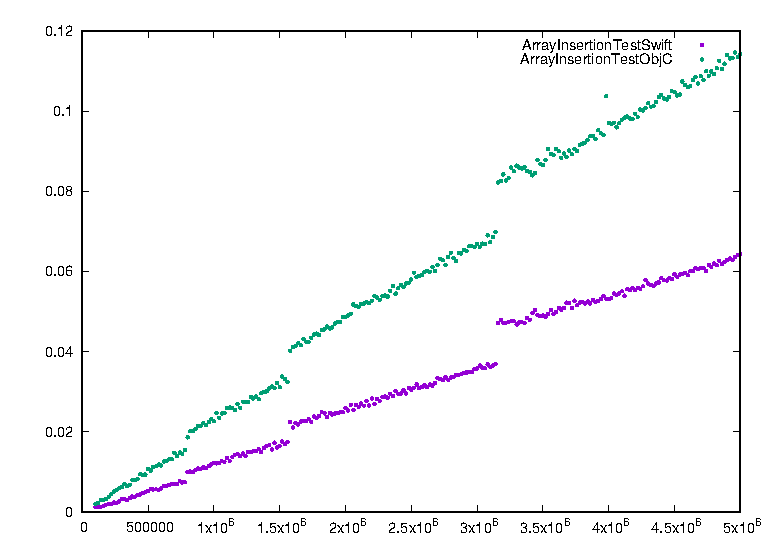
\includegraphics{plots/ArrayInsertion.eps}
    \caption{Wykres czasu działania testu ArrayInsertionTest dla obu języków}
    \label{p:array_insertion}
\end{figure}

\subsection{Analiza działania}

\begin{figure}
    \makebox[\textwidth][c]{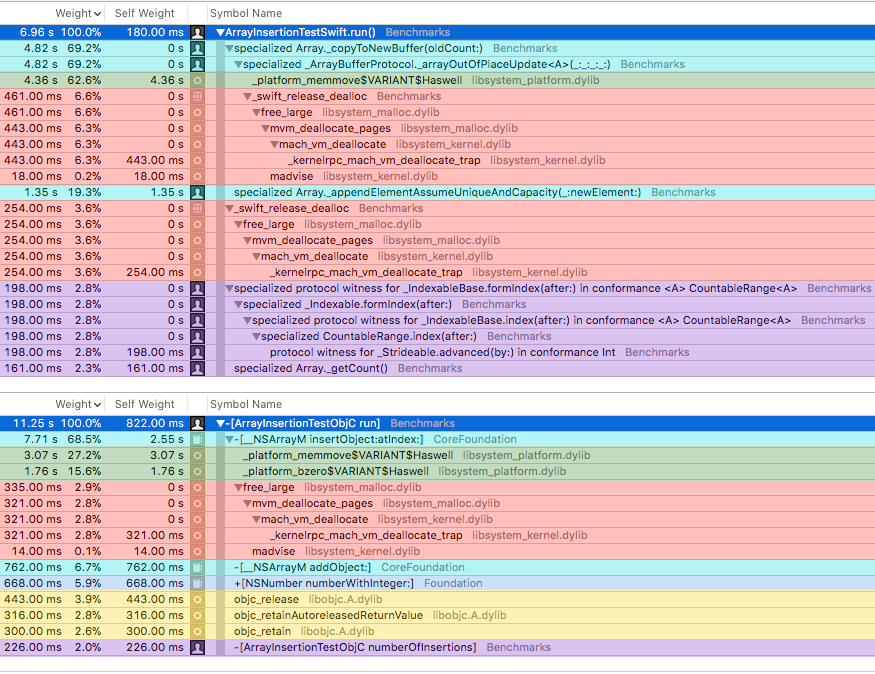
\includegraphics[width=1.3\textwidth]{img/ArrayInsertion.png}}
    \caption{Tablica profilowania dla testu ArrayInsertion (u góry - Swift, na dole - Objective-C)}
    \label{i:array_insertion}
\end{figure}

Rysunek \ref{i:array_insertion} przestawia wyniki profilowania w programie Instruments testu \texttt{ArrayInsertion} dla $n = 500000000$. Zgodnie z wykresem \ref{p:array_insertion}, czas działania testu w języku Objective-C jest około dwukrotnie dłuższy niż takiego samego testu w Swift. Tablica profilowania wskazuje jednak potencjalne powody takiego stanu:

\begin{itemize}
    \item Kod funkcji \objcinline{run} w teście języka Objective-C składa się z utworzenia modyfikowalnej tablicy (operacja ta ma znikomy czas, nie została wylistowana na tablicy profilowania) oraz zwykłej pętli \texttt{for} przebiegającej od 0 do \objcinline{numberOfInsertions}. W związku z tym można założyć, że czas działania pętli \texttt{for} to czas działania samej funkcji (oznaczony na tablicy profilownia jako \textit{Self Weight}) plus czas dostępu do właściwości \objcinline{numberOfInsertions} (kolor fioletowy na tablicy). Sumarycznie czas ten wynosi 1,05s. Kod testu dla języka Swift jest bardzo podobny, jedyną różnicą jest zastąpienie pętli \texttt{for} pętlą \texttt{for..in}, która w swojej implementacji używa protokołu \swiftinline{Indexable} i jego odpowiednich implementacji. Samo użycie tego protokołu wymaga 359 ms (instrukcje oznaczone kolorem fioletowym na tablicy profilowania), jednak czas działania samej funkcji \swiftinline{run} to zaledwie 180 ms, co daje łączny czas 539ms, czyli prawie o połowę krótszy niż w przypadku języka Objective-C. Zatem mimo, że pętle w języku Swift wydają się być bardziej skomplikowane, są wydajniejsze niż proste pętle \texttt{for} z Objective-C.
    \item W Objective-C kod funkcji \objcinline{addObject} został zinline'owany do wywołań metod \objcinline{insertObject:atIndex} oraz \objcinline{addObject} klas wewnętrznych. Łaczny czas wywołań tych dwóch metod to 3,31s. W Swift metoda \swiftinline{append} również została zinline'owana, tym razem do metod prywatnych \swiftinline{_copyToNewBuffer(oldCount:)} oraz \swiftinline{_appendElementAssumeUniqueAndCapacity(_:newElement:)}, łączny czas wywołania tych metod to jedynie 1,35 s. Można więc wyciągnąć wniosek, że sama implementacja tych metod jest mniej wydajna w Objective-C.
    \item Przenoszenie pamięci (kolor zielony na rysunku) trwa podobny czas w obu językach (4,36s dla Swift i 4,82 dla Objective-C). Jest to dosyć oczywiste, ze względu na fakt, że operacje na pamięci są wykonywane przez systemową bibliotekę \textsf{system\_platform}, zatem w dla obu języków została użyta ta sama implementacja, stąd czas jest podobny.
    \item Dealokowanie zajętej już pamięci (kolor czerwony na rysunku) zajmuje znacząco więcej czasu w Swift (715 ms) niż w Objective-C (335 ms). Powodem jednak nie jest sama implementacja procedury dealokowania, gdyż ta znajduje się w bibliotece \textsf{system\_malloc} i jest taka sama w obu językach, ale samo wykorzystanie mechanizmu dealokacji w obu językach.
    \item Jak wspomniano w rozdziale \ref{s:zarzadzanie_pamiecia}, ARC jest rozszerzeniem języka dodanym kilkanaście lat po premierze samego Objective-C, przez co w tablicy profilowania widnieją metody przeznaczone do tego zadania (kolor zółty na rysunku). Jak widać, ich wywołania zajmują około 10\% czasu wykonywania całego programu (1,05s)
    \item Tablice w Objective-C mogą zawierać tylko obiekty dziedziczące po klasie \objcinline{NSObject}. Typ całkowitoliczbowy, jest typem prostym, należy go zatem schować w obiekcie klasy \objcinline{NSNumber}, który można dodać do tablicy. Taka operacja to jednak dodatkowe 668ms do czasu działania programu (kolor niebieski).
\end{itemize}

\section{Rekurencyjne obliczanie liczby Fibonacciego}

Test polega na obliczeniu $n$-tej liczby Fibonacciego za pomocą naiwnego algorytmu rekurencyjnego. Kod obu testów znajduje się w plikach \texttt{FibonacciTest.m} oraz \texttt{FibonacciTest.swift}. Wyniki obu testów dla wartości $n \in <5, 40>$ zostały zwizualizowane na wykresie \ref{p:fibonacci}. Czas działania obu programów rośnie oczywiście wykładniczo, z wykresu wynika jednak, że program napisany w Swift jest około 40\% szybszy niż jego odpowiednik napisany w języku Objective-C.

\begin{figure}
    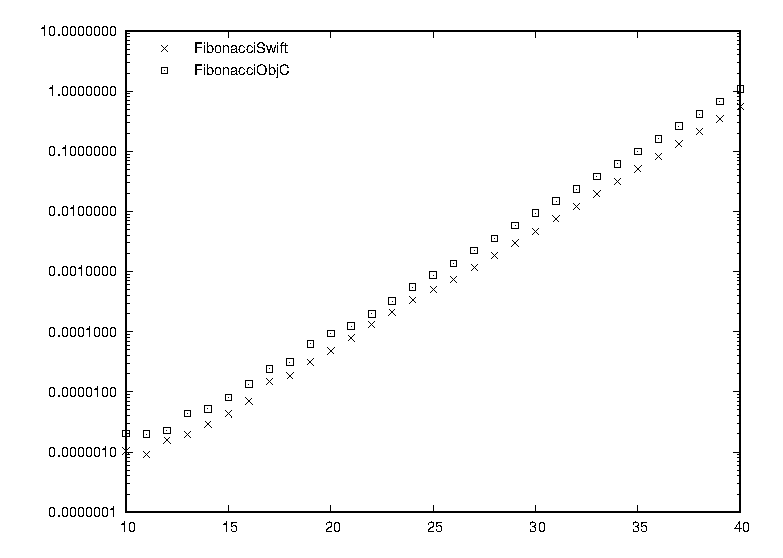
\includegraphics{plots/Fibonacci.eps}
    \caption{Wykres czasu działania testu FibonacciTest dla obu języków}
    \label{p:fibonacci}
\end{figure}

\subsection{Analiza działania}

\begin{figure}
    \makebox[\textwidth][c]{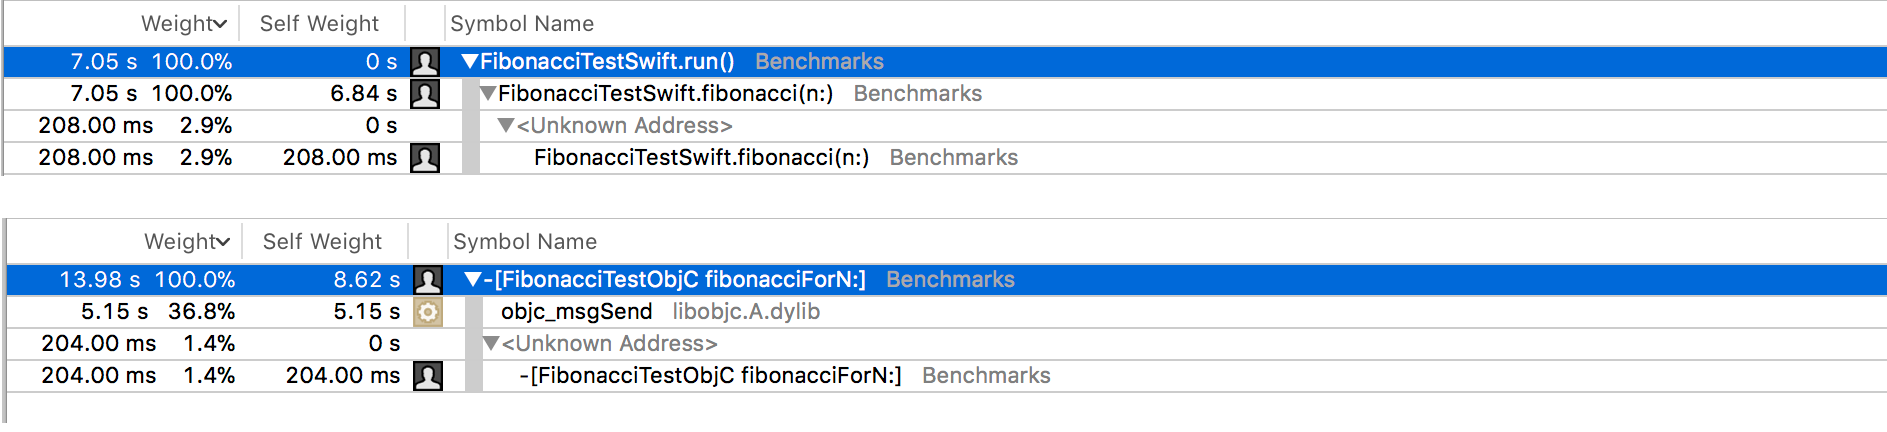
\includegraphics[width=1.3\textwidth]{img/Fibonacci.png}}
    \caption{Tablica profilowania dla testu ArrayInsertion (u góry - Swift, na dole - Objective-C)}
    \label{i:fibonacci}
\end{figure}

Tablica profilowania \ref{i:fibonacci} obu programów pozwala znaleźć powody różnicy prędkości pomiędzy dwoma językami. Główną różnicą jest wywołanie funkcji \objcinline{objc_msgSend } w teście napisanym w Objective-C. Wywołania te są odpowiedzialne za ponad 5 sekund czasu działania testu, co daje prawie 37\% całego czasu działania testu. Więcej o wywoływaniu metod w Objective-C napisano w sekcji \ref{s:system_typow}. Przykład ten dobrze obrazuje problemy z wydajnością języka Objective-C przy bardzo dużej ilości wywołań metod klas.

Drugim powodem, dla którego kod napisany w Objective-C jest wolniejszy jest samo działanie ciała metody \objcinline{[fibonacciForN:]}, które jest o ponad 2 sekundy wolniejsze od analogicznego kodu napisanego w Swift.

\section{Sortowanie bąbelkowe}
Sortowanie bąbelkowe to jeden z najprostszych algorytmów sortowania. Jego największą zaletą jest bardzo prosta i intuicyjna implementacja. Test opisany w tym rozdziale polega na zaimplementowaniu algorytmu sortowania bąbelkowego i uruchomieniu go na tablicy o wielkości $n \in <1000, 15000>$ wypełnionej losowymi 32-bitowymi liczbami całkowitymi.

Jak wynika z wykresu, implementacja w Swift jest ponad 10-krotnie szybsza niż najprostsza implementacja w Objective-C. Posortowanie tablicy $15000$ elementów zajmuje tylko $288 ms$ w przypadku kodu w Swift i $3,2 s$ dla Objective-C.

\subsection{Analiza działania}

Rysunek \ref{i:bubble_sort} przedstawia tablicę profilowania testu \texttt{BubbleSort} zaimplementowanego w języku Swifta (na górze) oraz w Objective-C (po środku) dla tablicy z 30000 elementów.

\begin{figure}
    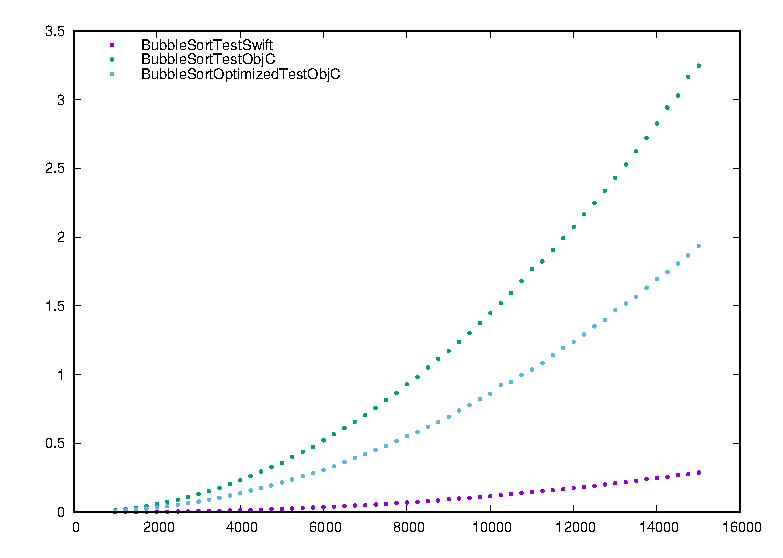
\includegraphics{plots/BubbleSort.eps}
    \caption{Wykres czasu działania testu BubbleSortTest dla obu języków}
    \label{p:bubble_sort}
\end{figure}

\begin{figure}
    \makebox[\textwidth][c]{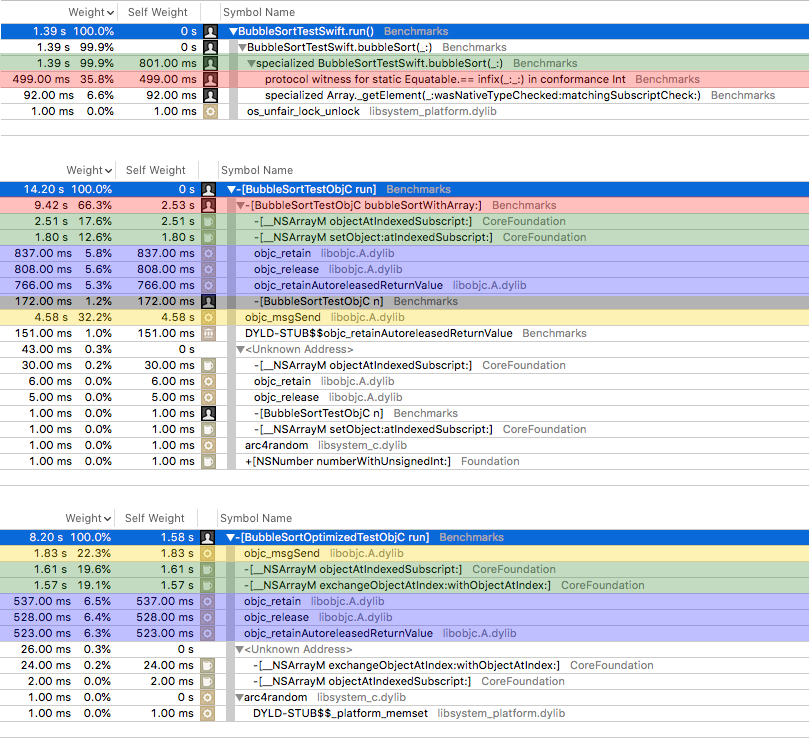
\includegraphics[width=1.3\textwidth]{img/BubbleSort.png}}
    \caption{Tablica profilowania dla testu BubbleSort (u góry - Swift, po środku - Objective-C, na dole - Objective-C po optymalizacjach)}
    \label{i:bubble_sort}
\end{figure}

Tablica profilowania testu napisanego w języku Swift jest bardzo krótka - aż 93\% czasu wykonywania testu zajęły dwie operacje:

\begin{itemize}
    \item około $0,5s$ zajęło porównywanie elementów w tablicy (oznaczone kolorem czerwonym)
    \item wywołanie operacji zdefiniowanych w samej metodzie \swiftinline{BubbleSort(:_)} zajęło około $800 ms$. Te operacje to obługa pętli \texttt{for} operacje arytmetyczne związane z przesuwaniem indeksów oraz zamiana elementów w tablicy.
\end{itemize}

Analiza implementacji w Objective-C jest nieco bardziej skomplikowana. Najwięcej czasu zajęło wysyłanie wiadomości do obiektów za pomocą metody \objcinline{objc_msgSend } (oznaczonej kolorem żółtym na tablicy profilowania). Czas wszystkich wywołań tej metody wyniósł $4,58s$.

Drugą najbardziej czasochłonną grupą opeacji były operacje odczytu i zapisu do/z tablicy (kolorem zielony na tablicy profilowania). Metody \objcinline{objectAtIndexedSubscript:} i \objcinline{setObject:atIndexedSubscript} są wywoływane po użyciu operatora indeksowania na tablicy \objcinline{NSArray} i łącznie czas ich wywołania zajmuje $4,31s$.

Wykonanie operacji z ciała metody \objcinline{run} (kolor czerwony), trwało łącznie $2,5s$. Operacje te to głównie obliczenia arytmetyczne oraz obsługa pętli \texttt{for}. Wywołania funkcji oznaczone kolorem niebieskim na tablicy profilowania dotyczą zarządzania licznikami referencji i łącznie również prawie $2,5s$.

Ciekawym przypadkiem pokazującym kosztowność systemu wysyłania wiadomości jest sprawdzanie wartości zapisanej do własciwości \objcinline{n}. W Objective-C dla każdej właściwości o nazwie \objcinline{x} kompilator generuje:

\begin{itemize}
    \item zmienną o nazwie \objcinline{_x}
    \item getter o nazwie \objcinline{x}
    \item setter \objcinline{setX:}
\end{itemize}

Z tego powodu, odczytanie wartości z właściwości  \objcinline{n} jest tak naprawdę wywołaniem metody \objcinline{n} i odczytanie wartości zmiennej ukrytej za właściwością. Z punktu widzenia kompilatora, odczyt taki jest zatem niczym innym niż wywołaniem metody, czyli wysłaniem wiadomości, stąd też samo odczytanie zmiennej zajmuje $172ms$ (kolor szary na tablicy profilowania).

Z powyższej analizy można łatwo wyznaczyć fragmenty kodu, które powinny zostać zoptymalizowane:

\begin{itemize}
    \item wywoływanie operatora indeksowania - zamiast zamieniać miejscami elementy za pomocą czterech wywołań operatora indeksowania, można użyć metody \objcinline{exchangeObjectAtIndex:withObjectAtIndex:} klasy \objcinline{NSArray}
    \item wysyłanie wiadomości do obiektów za pomocą \objcinline{objc_msgSend } - metoda \objcinline{exchangeObjectAtIndex:withObjectAtIndex:} jest za każdym razem wywoływana na tym samym obiekcie, dlatego też można już wcześniej wziąć wskaźnik na tą metodę (w nomenklaturze Objective-C - selektor), zachować referencję do niego i bezpośrednio wywoływać
    \item użycie właściwości \objcinline{n} - zamiast przy każdym sprawdzeniu warunku pętli odwoływać się do właściwości \objcinline{n}, można ją zachować na stosie jako zmienną lokalną funkcji i odwoływać się do niej bezpośrednio
\end{itemize}

Klasa \objcinline{BubbleSortOptimizedTestObjC} zawiera implementację wyżej wymienionych optymalizacji, wyniki działania zostały zawarte również na wykresie \ref{p:bubble_sort} oraz tablicy profilowania \ref{i:bubble_sort}. Jak widać, zaproponowane optymalizacje znacznie przyspieszyły działanie algorytmu o około $40\%$ względem kodu bez optymalizacji.

Największy przyrost wydajności zaobserwowano dla wywołań funkcji \objcinline{objc_msgSend }, czas $4,58s$ udało się zmniejszyć do $1,83s$ (spadek o $60\%$). Główne powody to zastąpienie kilku wywołań operatorów indeksowania jednym wywołaniem metody zamieniającej elementy miejscami oraz trzymanie referencji na tą metodę w zmiennej lokalnej. Spadł również czas wywołania metod związanych z operatorem indeksowania - pozbyto się zupełnie użycia metody ustawiającej wartość, a czas zużywany na metodę pobierającą wartość spadł z $2,51s$ do $1,61$. Łącznie czas operacji na tablicy spadł z $4,31s$ do $3,18s$ (spadek o $25\%$). Czas obsługi liczników referencji spadł z $2,4s$ do $1,6s$, co oznacza spadek o około $35\%$, a czas poświęcony wcześniej na odczyt właściwości \objcinline{n} spadła do wartości niezauważalnej podczas profilowania.

Pomimo tak znacznego przyspieszenia, kod ten nadal jest około 6-krotnie wolniejszy od implementacji w Swift.

\section{Budowanie binarnego drzewa poszukiwań}

Test opisany w tym rozdziale polega na utworzeniu binarnego drzewa poszukiwań o \swiftinline{n} elementach. Implementacja w języku Objective-C jest klasyczną implemenacją tego problemu. Zdefiniowana została struktura \objcinline{Node} przechowująca wskaźniki na lewe i prawe pod-węzeł oraz daną wartość.

Nieco ciekawiej wygląda kwestia implementacji algorytmu budowania drzewa w języku Swift. Po pierwsze, programości Swift często przedkładają bezpieczeństwo i niezawodność kodu nad jego wydajność. Przykładowo, zby zapewnić bezpieczeństwo dostępu do danych (np. podczas dostępu z wielu wątków) stosuje się struktury niemutowalne. Po drugie, Swift oferuje dużo więcej narzędzi niż Objective-C, m.in. funkcje wyższego rzędu jako \todo{Przetłumaczyć} \ang{first class citizens} czy algebraiczne typy danych w postaci typów wyliczeniowych z wartościami powiązanymi. Z tych dwóch powodów, poniższy test zawiera dwie implementacje w języku Swift. Obie zapewniają niemutowalność bieżących elementów drzewa - dodanie nowego elementu powoduje utworzenie nowego węzła, a nie zmodyfikowanie już istniejącego. Pierwsza implementacja to implementacja "klasyczna". Dane przechowywane są w klasie \swiftinline{Tree} (odpowiednik klasy \objcinline{Node} z Objective-C), a metoda dodająca element przechodzi po drzewie i tworzy nowy obiekt typu \swiftinline{Tree} w odpowiednim miejscu. Druga implementacja jest oparta na wykorzystaniu typów wyliczeniowych z wartościami powiązanymi i wygląda nieco bardziej jak kod znany z języków funkcyjnych. Dane przechowywane są tutaj w typie wyliczeniowym \swiftinline{Tree}, który definiuje dwa "konstruktory typów": \swiftinline{empty} oraz \swiftinline{node(Tree, Int, Tree)}. Funkcja dodająca element używa pattern matchingu, aby znaleźć odpowiednie miejsce w drzewie i tam dodaje nowy obiekt. Kod opisanych testów znajduje się odpowiednio w plikach \texttt{BinarySearchTreeTest.m}, \texttt{BinarySearchTreeClassicTest.swift} oraz \texttt{BinarySearchTreeEnumsTest.swift}.

\subsection{Analiza działania}

\begin{figure}
    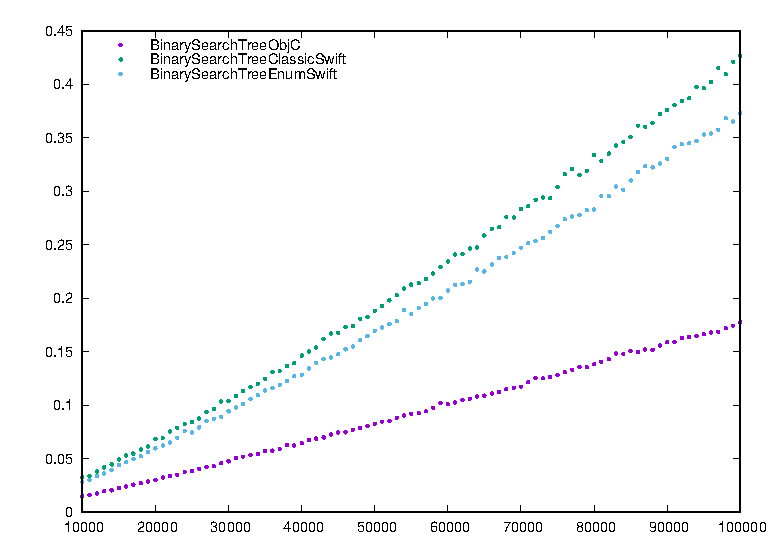
\includegraphics{plots/BinarySearchTree.eps}
    \caption{Wykres czasu działania testu BinarySearchTree}
    \label{p:binary_search}
\end{figure}

Wykres \ref{p:binary_search} Przedstawia wyniki działania testu tworzącego drzewo binarne o wielkości \swiftinline{n}. Jak widać, jest to pierwszy test, którym implementacja w Objective-C jest szybsza od implementacji w Swift. Kod napisany w starszym z języków wykonuje się około 2 razy szybciej od implementacji napisanej Swift przy pomocy typów wyliczeniowych i ponad dwa razy szybciej od "klasycznej" implementacji w Swift. 

\begin{figure}
    \makebox[\textwidth][c]{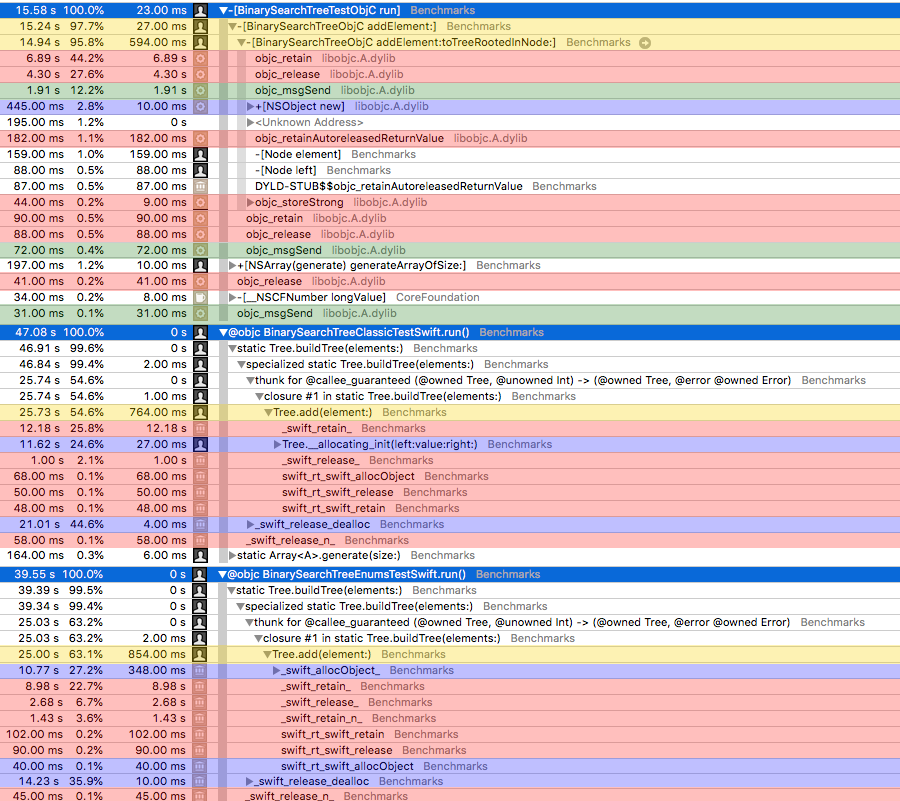
\includegraphics[width=1.3\textwidth]{img/BinarySearch.png}}
    \caption{Tablica profilowania dla testu BinarySearchTree (u góry - Objective-C, po środku - Swift przy użyciu klas, na dole - Swift przy użyciu typów wyliczeniowych)}
    \label{i:binary_search}
\end{figure}

Rysunek \ref{i:binary_search} przestawia tabelę profilowania ww. testów dla wejściowego rozmiaru drzewa \swiftinline{n = 5000000}. Dla czytelności pominięte zostały wpisy, których czas wykonywania nie przekraczał $0.1\%$ łącznego czasu wykonywania testu. Podczas tego pojedynczego uruchomienia kod napisany w Objective-C okazał się być aż 2,5 raza szybszy od implementacji w Swift przy użyciu typów wyliczeniowych oraz 3 razy szybszy od klasycznej implementacji w Swift. Głównym powodem takiego stanu rzeczy była wspomniana we wstępie do tego testu niemutowalność struktury drzewa dla implementacji w Swift. 

Największą ilość czasu podczas wykonywania testów w Swift zajęło tworzenie nowych obiektów (kolor niebieski na tablicy profilowania) oraz obsługa ARC (kolor czerwony). Powodem, dla którego tak się działo jest wielokrotne tworzenie obiektów dla tych samych węzłów, co powodowało bardzo częste wywoływania inicjalizatora i deinicjlizatora oraz w późniejszym etapie funkcji odpowiadających za inkrementację i dekrementację licznika referencji. Dla implementacji w Swifta z użyciem typów wyliczeniowych łączny czas wywołań inicjalizatorów i deinicjalizatorów wyniósł 25,04s, a operacje obługi liczników referencji zajęły łącznie 13,33s. Dla kodu napisanego za pomocą klas w Swift wartości te wynosiły odpowiednio 32,63s dla inicjalizacji i deinicjalizacji oraz 12,41s dla obsługi ARC. W Objective-C czas tworzenia nowych obiektów wynosił zaledwie 445ms. Obsługa ARC zajęła łącznie ok 11,64s. Dodatkowo do czasu działania kodu Objective-C należy dodać standardowo czas przesyłania metod za pomocą funkcji \objcinline{objc_msgSend}, który wyniósł 2,01s.

Z powyższej analizy wynika, że choć w Swift można napisać bardzo bezpieczny kod, to ma to jednak swoją cenę w postaci mocno obniżonej wydajności. Analiza nie byłaby jednak pełna, jeśli nie zostałaby przeprowadzona próba napisania kod działającego identycznie jak kod Objective-C, tj. modyfikująca aktualne węzły w drzewie. 

\begin{figure}
    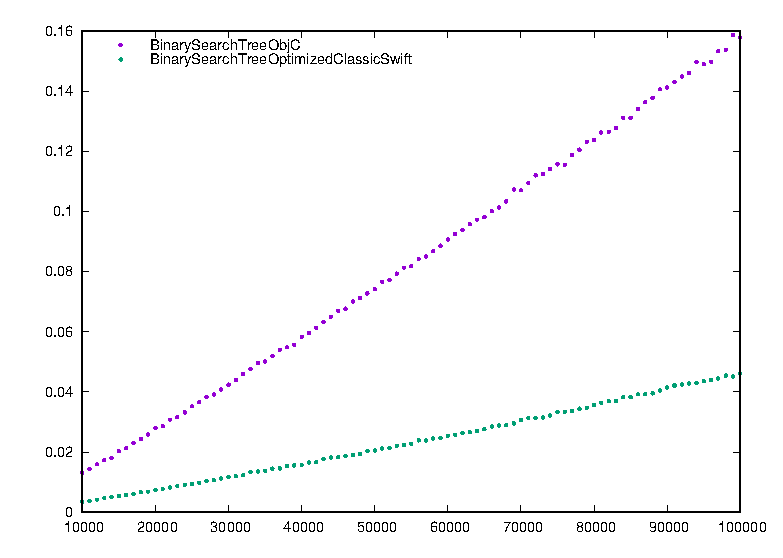
\includegraphics{plots/BinarySearchTree2.eps}
    \caption{Wykres czasu zoptymalizowanej wersji w Swift dla BinarySearchTree w porównaniu z wersją w Objective-C}
    \label{p:binary_search2}
\end{figure}

\begin{figure}
    \makebox[\textwidth][c]{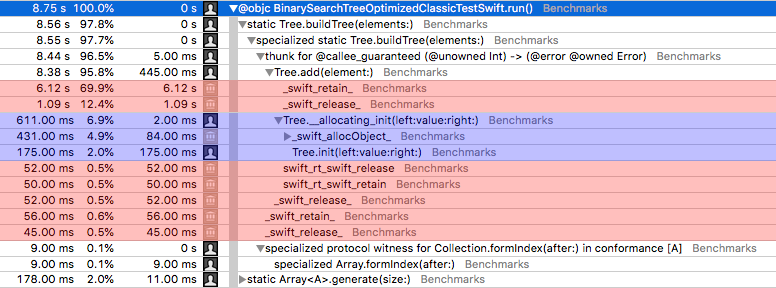
\includegraphics[width=1.3\textwidth]{img/BinarySearch2.png}}
    \caption{Tablica profilowania dla zoptymalizowanej wersji testu BinarySearchTree}
    \label{i:binary_search2}
\end{figure}

Wykres \ref{p:binary_search2} przedstawia czas działania zoptymalizowanego testu napisanego w języku Swift. Jak widać, test ten jest teraz około 3-krotnie szybszy od testu zaimplementowanego w Objective-C. Tablica profilowania \ref{i:binary_search2} tego testu wskazuje wyraźnie na przyczynę poprawy wydajności. W zoptymalizowanej implementacji pozbyto się tworzenia dużej ilości nowych obiektów podczas dodawania nowego elementu. Wywołania inicjalizatora zajmują teraz jedynie 611ms, co oznacza co oznacza skrócenie czasu potrzebnego na inicjalizację obiektów o 98\% (wcześniej - 32,63s). Czas obsługi ARC również uległ zmniejszeniu - z 11,64s do 7,47s (spadek o 35\%). 

Zatem pomimo początkowych problemów z wydajnością również i w tym teście kod napisany w Swift okazał się szybszy. Należy jednak uważać, z jakich właściwości języka się korzysta. Pisanie kodu w oparciu o idee zaczerpnięte z programowania funkcyjnego może nie być dobrym wyborem pod względem wydajności kodu.

\section{Rodzaje wywołania metod}

Język Swift obsługuje dwa rodzaje wywołań metod: statyczną (\ang{direct dispatch}) i dynamiczną (\ang{table dispatch}). Oprócz tego, ze względu na możliwość użycia kodu Swift w Objective-C, programista może również używać wywoływania poprzez wiadomości (\ang{message dispatch}), które jest domyślnym sposobem wywoływania w starszym z języków.

Wywoływanie statyczne jest uznawane za najszybszy sposób wykonywania metod. Główną cechą jest pełna wiedza o tym, która metoda ma zostać wykonana już w trakcie procesu kompilowania. Z tego powodu, kompilator może stosować dużą ilość optymalizacji, takich jak bezpośrednie odwołania do adresu funkcji czy wywołanie funkcji "w linii" (\ang{inline}). Główną jej wadą jest natomiast bardzo ograniczone wsparcie dla polimorfizmu, przez co większość języków implementuje dodatkowo inny rodzaj wywoływania metod (np. tablice wirtualne w C++). W Swift wywoływanie statyczne jest używane dla struktur oraz rozszerzeń protokołów (\ang{protocol extensions}).

Wywołanie dynamiczne to mechanizm zaimplementowany w większości współczesnych obiektowych języków programowania. Jego działanie opiera się głównie o tablice wirtualne. W Swift istnieją dwa rodzaje tablic wirtualnych:

\begin{itemize}
    \item \textit{virtual dispatch tables} - tablice wirtualne tworzone dla klas i służące do wywoływania odpowiednich metod klasy. Dzięki nim, możliwe jest dziedziczenie i przeładowywanie metod w klasach dziedziczących.
    \item \textit{witness tables} - tablice wirtualne tworzone dla każdego typu implementującego protokół. Dzięki nim możliwe jest użycie protokołów.
\end{itemize}

Zaletą takiego podejścia jest jego elastyczność, która umożliwia zaimplementowanie takich elementów języka, jak dziedziczenie czy protokoły. Wadą natomiast jest dodatkowy czas, potrzebny na wyszukanie adresu funkcji w tablicy wirtualnej. Uniemożliwia też stosowanie niektórych metod optymalizacji kodu. W Swift wywoływanie dynamiczne jest domyślnie używane dla klas oraz protokołów.

Wywołanie przez wiadomości to mechanizm odziedziczony z Objective-C i używany głównie w trakcie wywoływania kodu Objective-C. Jest uważany za najwolniejszy z trzech dostępnych sposobów wywoływania funkcji, wspiera jednak funkcje języka, takie jak selector czy KVO (\ang{Key Value Observers}) bez których prawie niemożliwe byłoby używanie klas i bibliotek napisanych w Objective-C z poziomy kodu swiftowego.

Test opisany w tym rozdziale polega na wykonaniu bardzo prostej funkcji mnożącej liczbę całkowitą przez 2 na kilka sposobów:

\begin{itemize}
    \item jako metoda struktury - metoda struktury zostanie wywołana statycznie. Kod tego eksperymentu znajduje się w teście \swiftinline{StaticDispatchTest.swift}.
    \item jako metoda struktury implementującej protokół - ze względu na fakt, że struktura jest schowana za protokołem i kompilator nie ma sposobu na zidentyfikowanie dokładnego typu obiektu, metoda zostanie wywołana dynamicznie. Kod dla tego eksperymentu znajduje się w teście \swiftinline{DynamicDispatchTest.swift}.
    \item jako metoda klasy z Objective-C - funkcje napisane w Objective-C są wywoływane przez wysłanie wiadomości. Kod dla tego testu znajduje się w pliku \swiftinline{MessageDispatchTest.mm}.
\end{itemize}

\subsection{Analiza działania}

Wyniki wyżej opisanych testów znajdują się na wykresie \ref{p:dispatch_method}.

\begin{figure}
    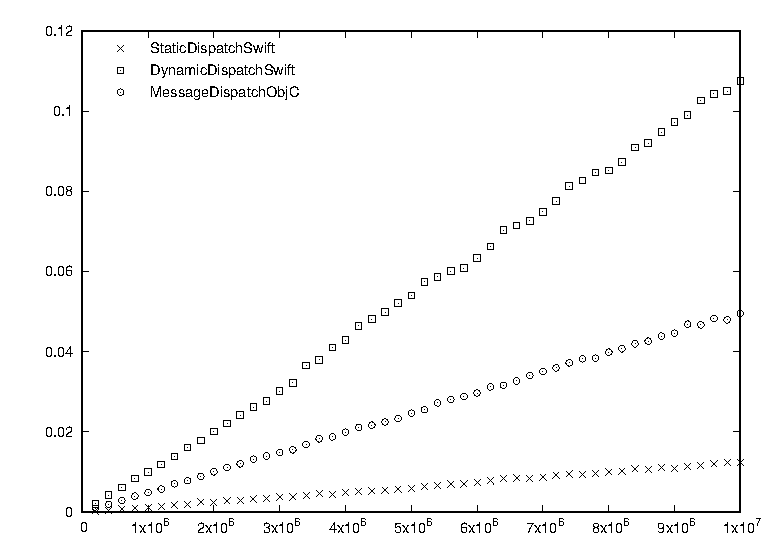
\includegraphics{plots/Dispatch.eps}
    \caption{Wykres czasu działania trzech metod wywołania funkcji: statycznej, dynamicznej i przez wiadomości}
    \label{p:dispatch_method}
\end{figure}

Jak widać na wykresie, czasy działania różnych metod wywołania różnią się od siebie znacznie. Zgodnie z przewidywaniami z opisu tego testu, statyczna metoda wywołania funkcji jest najszybsza. Na drugim miejscu znalazł się mechanizm wywoływania przez wiadomości, który jest ok. 4-krotnie wolniejszy od wywoływania statycznego. Wywołanie dynamiczne okazało sie natomiast niespodziewanie wolne, zajęło ponad 2 razy więcej czasu niż wywołanie przez wiadomości i prawie 9 razy więcej od wywołania statycznego. Tablica profilowania z rysunku \ref{i:dispatch_method} wskazuje na pewne powody takiego stanu.

\begin{figure}
    \makebox[\textwidth][c]{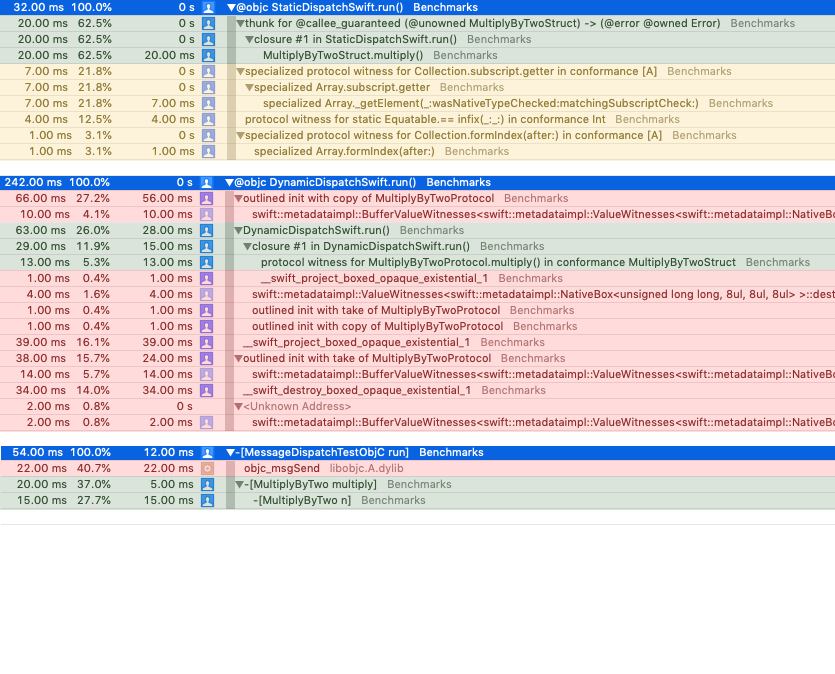
\includegraphics[width=1.3\textwidth]{img/DispatchMethod.png}}
    \caption{Tablica profilowania dla testów mechanizmów wywołania funkcji: statycznego (u góry), dynamicznego (w środku) i przez wiadomości (na dole)}
    \label{i:dispatch_method}
\end{figure}

Tablica profilowania przedstawiona na rysunku \ref{i:dispatch_method} przedstawia czas działania testów dla różnych metod wywołania i parametru wejściowego $n = 20000000$. Na jej podstawie można wysnuć kilka wniosków odnośnie czasu działania testów.

Po pierwsze, na czas działania testu dla wywołania statycznego składa się jedynie obsługa pętli \swiftinline{forEach} (kolor żółty na tablcy profilowania) oraz wywołanie funkcji \swiftinline{multiply}. To właśnie brak dodatkowych kosztownych operacji powoduje, że wywołanie statyczne jest najszybszym z trzech porównywanych mechanizmów.

Przy wywołaniu dynamicznym, implementacja funkcji \swiftinline{multiply} jest schowana za protokołem. Z tego powodu, kompilator musi w trakcie działania programu znaleźć adres do odpowiedniej implementacji, którą należy wywołać. Operacja ta zostanie wykonana w dwóch krokach:

\begin{itemize}
    \item najpierw kompilator utworzy tablicę wirtualną \ang{Witness table} dla protokołu \swiftinline{MultiplyByTwoProtocol} oraz struktury \swiftinline{MultiplyByTwoStruct}. Tablica ta zawiera odnośniki do adresów funkcji dla typu implementującego dany protokół. W tym przypadku znajdzie się tam adres implentacji dla funkcji \swiftinline{multiply} w strukturze \swiftinline{MultiplybyTwoStruct}.
    \item następnie kompilator powiąże utworzoną tablicę z danym obiektem struktury tworząć tymczasowy typ egzystencyjny (\ang{existential type}). Taki obiekt zostanie dopiero przekazany do wywołania funkcji.
\end{itemize}

Z tablicy profilowania wynika, że tworzenie tablicy \textit{Witness table} zajmuje 110ms, a tworzenie i usuwanie typu egzystencjalnego to czas 73ms, co łącznie daje aż 75\% całego czasu wykonania funkcji (kolor czerwony na tablicy profilowania).

Wywołanie przez wiadomości okazało się szybsze niż wywołanie dynamiczne. Zawdzięcza to głównie świetnej optymalizacji oraz użyciu cache do przechowywania informacji o tym, jaka wiadomość powinna zostać wysłana. Jako, że wysyłana jest cały czas taka sama wiadomość do tej samej klasy, to cache jest tutaj bardzo wydajną formą optymalizacji. Nadal jednak narzut czasowy powodowany przez wywołania funkcji \objcinline{objc_msgSend} to 22ms, czyli około 40\% czasu wykonywania całej metody.





% \begin{itemize}  
    % \item wywołanie dynamiczne wymaga sprawdzania w trakcie działania programu, która funkcja powinna zostać wywołana, powoduje to dodatkowy narzut czasowy, który dla powyższego testu wynosił ok. 102ms (kolor czerwony na tablicy profilowania).
    % \item do zaimplementowania testu do wywołania dynamicznego użyto klasy. Klasy w języku Swift są typem referencyjnym, co oznacza, że pamięć dla nich jest zawsze alkowanay na stercie, a co za tym idzie, wymagają obsługi zliczania referencji. W powyższym teście koszt obługi liczników referencji był największą składową tego testu, łącznie zajął ok. 311ms, czyli 66\% całkowitego czasu działania testu (kolor niebieski na tablicy profilowania).
% \end{itemize}




%%%%% BIBLIOGRAFIA

%\begin{thebibliography}{1}
%\bibitem{example} \ldots
%\end{thebibliography}                                                                                                                                                          

\end{document}
